\section{Decider for backward reasoning}\label{sec:backward-reasoning}

\begin{figure}
  \centering
  \begin{subfigure}[m]{0.45\textwidth}
    \centering
    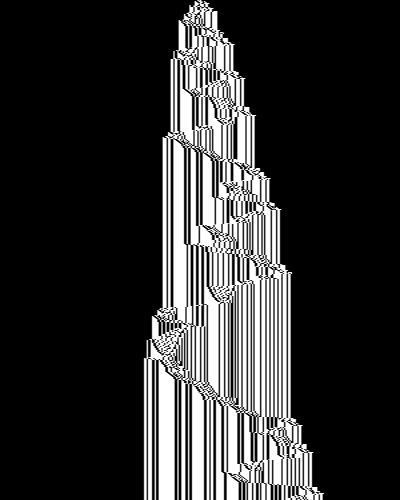
\includegraphics[width=\textwidth]{space-time-diagrams/backward_reasoning_55897188.png}
    \caption{10,000-step space-time diagram of bbchallenge's machine \#55,897,188. \url{https://bbchallenge.org/55897188}}
    \label{fig:y equals x}
  \end{subfigure}
  \hfill
  \begin{subfigure}[m]{0.45\textwidth}
    \centering
    \begin{tabular}{lll}
                            & 0                       & 1   \\
      \textcolor{colorA}{A} & 1R\textcolor{colorB}{B} & 0LD \\
      \textcolor{colorB}{B} & 1L\textcolor{colorC}{C} & 0RE \\
      \textcolor{colorC}{C} & - - -                   & 1LD \\
      D                     & 1LA                     & 1LD \\
      E                     & 1RA                     & 0RA
    \end{tabular}


    \caption{Transition table of machine \#55,897,188.}

  \end{subfigure}

  \begin{subfigure}[m]{1\textwidth}
    \vspace{5ex}
    \centering
    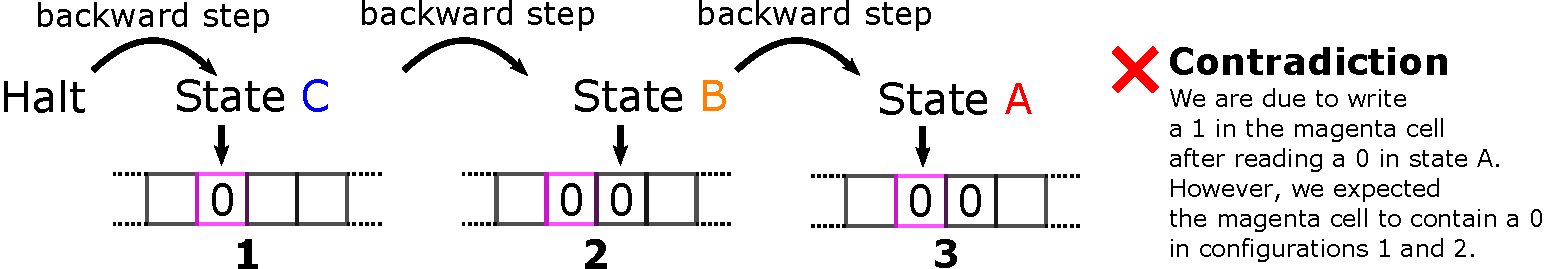
\includegraphics[width=0.9\textwidth]{backward-reasoning.pdf}

    \caption{Contradiction reached after 3 backward steps: machine \#55,897,188 does cannot reach its halting configuration hence it does not halt.}

  \end{subfigure}

  \caption{Applying backward reasoning on bbchallenge's machine \#55,897,188. (a) 10,000-step space-time diagram of machine \#55,897,188. The \textit{forward} behavior of the machine looks very complex. (b) Transition table. (c) We are able to deduce that the machine will never halt thanks to only 3 backward reasoning steps: because a contradiction is met, it is impossible to reach the halting configuration in more than 3 steps -- and, by (a), the machine can do at least 20,000 without halting starting from all-0 tape.}
  \label{fig:backward-reasoning}
\end{figure}


Backward reasoning, as described in \cite{Marxen_1998}, takes a different approach than what has been done with deciders in Sections~\ref{sec:cyclers} and \ref{sec:translated-cyclers}. Indeed, instead of trying to recognise a particular kind of machine's behavior, the idea of backward reasoning is to show that, independently of the machine's behavior, the halting configurations are not reachable. In order to do so, the decider simulates the machine \textit{backwards} from halting configurations until it reaches some obvious contradiction.

Figure~\ref{fig:backward-reasoning} illustrates this idea on bbchallenge's machine \#55,897,188. From the space-time diagram, the \textit{forward} behavior of the machine from all-0 tape looks to be extremely complex, Figure~\ref{fig:backward-reasoning}a. However, by reconstructing the sequence of transitions that would lead to the halting configuration (reading a 0 in state \textcolor{colorC}{C}), we reach a contradiction in only 3 steps, Figure~\ref{fig:backward-reasoning}c. Indeed, the only way to reach state  \textcolor{colorC}{C} is to come from the right in state \textcolor{colorB}{B} where we read a 0. The only way to reach state \textcolor{colorB}{B} is to com from left in state  \textcolor{colorA}{A} where we read a 0. However, the transition table (Figure~\ref{fig:backward-reasoning}b) is instructing us to write a 1 in that case, which is not consistent with the 0 that we assumed was at position in order for the machine to halt.

Backward reasoning in the case of Figure~\ref{fig:backward-reasoning} was particularly simple because there was only one possible previous configuration for each backward step -- e.g. there is only one transition that can reach state \textcolor{colorC}{C} and same for state \textcolor{colorB}{B}. In general, this is not the case and the structure created by backward reasoning is a tree of configurations instead of just a chain. If all the leaves of a backward reasoning tree of depth $D$ reach a contradiction, we know that if the machine runs for $D$ steps from all-0 tape then the machine cannot reach a halting configuration and thus does not halt.

\subsection{Pseudocode}

\begin{algorithm}
  \caption{{\sc decider-backward-reasoning}}\label{alg:backward-reasoning}

  \begin{algorithmic}[1]
    \State{\textbf{const int} RIGHT, LEFT = 0, 1}
    \State \textbf{struct} Transition \{
    \State \tabi\textbf{int} state, read, write, move
    \State \}
    \State \textbf{struct} Configuration \{
    \State \tabi\textbf{int} state
    \State \tabi\textbf{int} headPosition
    \State \tabi\textbf{int $\boldsymbol{\to}$ int} tape
    \State \tabi\textbf{int} depth
    \State \}

    \State

    \Procedure{\textbf{Configuration} {\sc apply-transition-backwards}}{\textbf{Configuration} conf,\textbf{Transition} t}
    \State \textbf{int} reversedHeadMoveOffset = (t.move == RIGHT) ? -1 : 1
    \State \textbf{int} previousPosition = conf.headPosition+reversedHeadMoveOffset
    \State // Backward contradiction spotted
    \If{previousPosition \textbf{in} conf.tape \textbf{and} conf.tape[previousPosition] != t.write}
    \State \textbf{return} \textbf{nil}
    \EndIf
    \State \textbf{Configuration} previousConf = \{.state = t.state, .depth = conf.depth + 1, .tape = conf.tape\}
    \State previousConf.headPosition = previousPosition
    \State previousConf.tape[previousPosition] = t.read
    \State \textbf{return} previousConf
    \EndProcedure
    \State
    \Procedure{\textbf{bool} {\sc decider-backward-reasoning}}{\textbf{TM} machine,\textbf{int} maxDepth}

    \State \textbf{Stack$\boldsymbol{<}$Configuration$\boldsymbol{>}$} configurationStack
    \For{\textbf{int} (state,read) \textbf{in} {\sc get-undefined-transitions}(machine)}
    \State \textbf{Configuration} haltingConfiguration = \{.state = state,.depth=0,.headPosition = 0\}
    \State haltingConfiguration.tape = \{0: read\}
    \State configurationStack.\textbf{push}(haltingConfiguration)
    \EndFor
    \State \textbf{Set$\boldsymbol{<}$Configuration$\boldsymbol{>}$} configurationsSeen = \{\}
    \While{!configurationStack.\textbf{empty}()}
    \State \textbf{Configuration} currConf = configurationStack.\textbf{pop}()
    \If{currConf.depth $>$ maxDepth} \textbf{return} false \EndIf
    \If{ currConf \textbf{in} configurationsSeen} \textbf{continue} \EndIf
    \State configurationsSeen.\textbf{insert}(currConf)
    \State \textbf{List$\boldsymbol{<}$Configuration$\boldsymbol{>}$} confList = []

    \For{\textbf{Transition} transition \textbf{in} {\sc get-transitions-reaching-state}(machine,currConf.state)}
    \State \textbf{Configuration} previousConf = {\sc apply-transition-backwards}(currConf, transition)
    \State // If no contradiction
    \If{previousConf != \textbf{nil}}
    \State configurationStack.\textbf{push}(previousConf)
    \EndIf
    \EndFor
    \EndWhile

    \State \textbf{return} true
    \EndProcedure

  \end{algorithmic}
\end{algorithm}

We assume that we are given routine {\sc get-undefined-transitions}(machine) which returns the list of (state,readSymbol) pairs of all the undefined transitions in the machine's transition table, for instance [(\textcolor{colorC}{C},0)] for the machine of Figure~\ref{fig:backward-reasoning}b. We also assume that we are given routine {\sc get-transitions-reaching-state}(machine,targetState) which returns the list of all machine's transitions that go to the specified target state, for instance [(\textcolor{colorA}{A},1,0LD),(\textcolor{colorC}{C},1,1LD),(D,1,1LD)] for target state D in the machine of Figure~\ref{fig:backward-reasoning}b. These two routines contain very minimal logic as they only lookup in the description of the machine for the required information.

\subsection{Correctness}

\begin{theorem}\label{th:backward-reasoning}\normalfont
  Let $\mathcal{M}$ be a Turing machine and $D\in\mathbb{N}$.
  Then, {\sc decider-backward-reasoning}($\mathcal{M}$,$D$) returns \texttt{true} if and only if no undefined transition of $\mathcal{M}$ can be reached in more than $D$ steps.
\end{theorem}
\begin{proof}
  The tree of backward configurations is maintained in a DFS fashion through a stack (Algorithm~\ref{alg:backward-reasoning}, l.24). Initially, the stack is filled with the configurations where only one tape cell is defined and state is set such that the corresponding transition is undefined (i.e. the machine halts after that step), l.25-28.

  Then, the main loop runs until either (a) the stack is empty or (b) one leaf exceeded the maximum allowed depth, l.30 and l.32. Note that running the algorithm with increased maximum depth increases its chances to contradict all branches of the backward simulation tree. At each step of loop, we remove the current configuration from the stack and we try to apply all the transitions that leads to its state backwards by calling routine {\sc apply-transition-backwards}(configuration, transition).

  The only case where it is not possible to apply a transition backwards, i.e. the case where a contradiction is reached is when the tape symbol at the position where the transition comes from (i.e. to the right if transition movement is left and vice-versa) is defined but is not equal to the write instruction of the transition. Indeed, that means that the future (i.e. previous backward steps) is not consistent the current transition's write instruction. This logic is checked l.16. Otherwise, we can construct the previous configuration (i.e. next backward step) and augment depth by 1. We then stack this configuration in the main routine (l.39).

  The algorithm returns \texttt{true} if and only if the stack ever becomes empty which means that all leaves of the backward simulation tree of depth $D$ have reached a contradiction and thus, no undefined transition of the machine is reachable in more than $D$ steps.

  This pseudocode contains a slight optimisation with the use of set \texttt{configurationSeen} (l.29). This set racks configurations which would have already been seen in different branches of the tree in order not traverse them twice (l.32-33). While not needed in theory, this optimisation is useful in practice, especially at large depths (e.g. $D=300$).
\end{proof}

\begin{corollary}\normalfont
  Let $\mathcal{M}$ be a Turing machine and $D\in\mathbb{N}$. If {\sc decider-backward-reasoning}($\mathcal{M}$,$D$) returns \texttt{true} and machine $\mathcal{M}$ can run $D$ steps from all-0 tape without halting then the behavior of $\mathcal{M}$ from all-0 tape has been decided: $\mathcal{M}$ does not halt.
\end{corollary}
\begin{proof}
  By Theorem~\ref{th:backward-reasoning} we know that no undefined transition of $\mathcal{M}$ can be reached in more than $D$ steps. Hence, if machine $\mathcal{M}$ can run $D$ steps from all-0 tape without halting, it will be able to run the next $D+1^{\text{th}}$ step. From there, the machine cannot halt or it would contradict the fact that halting trajectories have at most $D$ steps. Hence, $\mathcal{M}$ does not halt from all-0 tape.
\end{proof}

\subsection{Results}

The decider was coded in \texttt{golang} and is accessible at this link: \url{https://github.com/bbchallenge/bbchallenge-deciders/blob/main/decider-backward-reasoning}. Note that collaborative work allowed to find a bug in the initial algorithm that was implemented\footnote{Thanks to collaborators \url{https://github.com/atticuscull} and \url{https://github.com/modderme123}.}.

The decider decided 2,243,340 machines, out of 3,574,222 machines that were left after deciders for ``Cyclers'' and ``Translated Cyclers'' (Section~\ref{sec:cyclers} and Section~\ref{th:translated-cyclers}). Maximum depth was set to 300. More information about these results are available at: \url{https://discuss.bbchallenge.org/t/decider-backward-reasoning/35}.
